% !TEX encoding = UTF-8 Unicode
\documentclass{beamer}

\usepackage{amsmath}
\usepackage{color}
\usepackage{fancyvrb}
\usepackage{gensymb}
\usepackage{graphicx}
\usepackage{hyperref}
\usepackage{textcomp}
\usepackage{tikz}

\usetikzlibrary{arrows,positioning,shapes,shapes.multipart} 
\tikzstyle{every picture}+=[remember picture]

\definecolor{mygreen}{rgb}{0.88,0.95,0.88}

\usetheme{Warsaw}

\newcommand{\btVFill}{\vskip0pt plus 1filll}

\title[Data Visualization with R - Tidyverse tutorial]{Data Visualization with R \\ Tidyverse tutorial}
\author{Ariane Ducellier}
\date{University of Washington - Fall 2024}

\begin{document}

	\begin{frame}
		\titlepage
	\end{frame}

	\begin{frame}[fragile]
		\frametitle{What is tidyverse?}

		A collection of R packages designed for data science.

		\vspace{1em}

		Basic packages:
		\begin{itemize}
			\item \textbf{ggplot2:} graphics
			\item \textbf{dplyr:} data manipulation
			\item \textbf{tidyr:} getting to tidy data
			\item \textbf{readr:} reading rectangular data (e.g. csv, tsv, fwf)
			\item \textbf{purrr:} working with functions and vectors
			\item \textbf{tibble:} a modern re-imagining of the data frame
			\item \textbf{stringr:} working with strings
			\item \textbf{forcats:} working with R factors to handle categorical variables
		\end{itemize}

		\vspace{1em}

		Additional packages associated to \verb|tidyverse| need to be installed and loaded separately to import data, wrangle data, program and model.		
		
	\end{frame}

	\begin{frame}
		\frametitle{Main concepts of data wrangling}

		\begin{itemize}
		\setlength{\itemsep}{1em}
			\item Understand.
			\item Format $\rightarrow$ Produce tidy data:
			\begin{itemize}
				\item Every column is a variable.
				\item Every row is an observation.
				\item Every cell is a single value.
			\end{itemize}
			\item Clean.
			\item Enrich.
			\item Validate.
			\item Analysis / Model $\rightarrow$ In our case, we are going to produce visuals to communicate information on the dataset to the viewer.
		\end{itemize}

	\end{frame}

	\begin{frame}
		\frametitle{Benefits of data wrangling}

		\begin{itemize}
			\item Organized and easily understandable data.
			\item Faster results.
			\item Better data flow for modeling or data visualization.
			\item Easier aggregation for insight extraction.
			\item Data quality.
			\item Data enriching.
		\end{itemize}

	\end{frame}

	\begin{frame}
		\frametitle{Frameworks in Data Science: KDD}

		Knowledge Discovery in Databases

		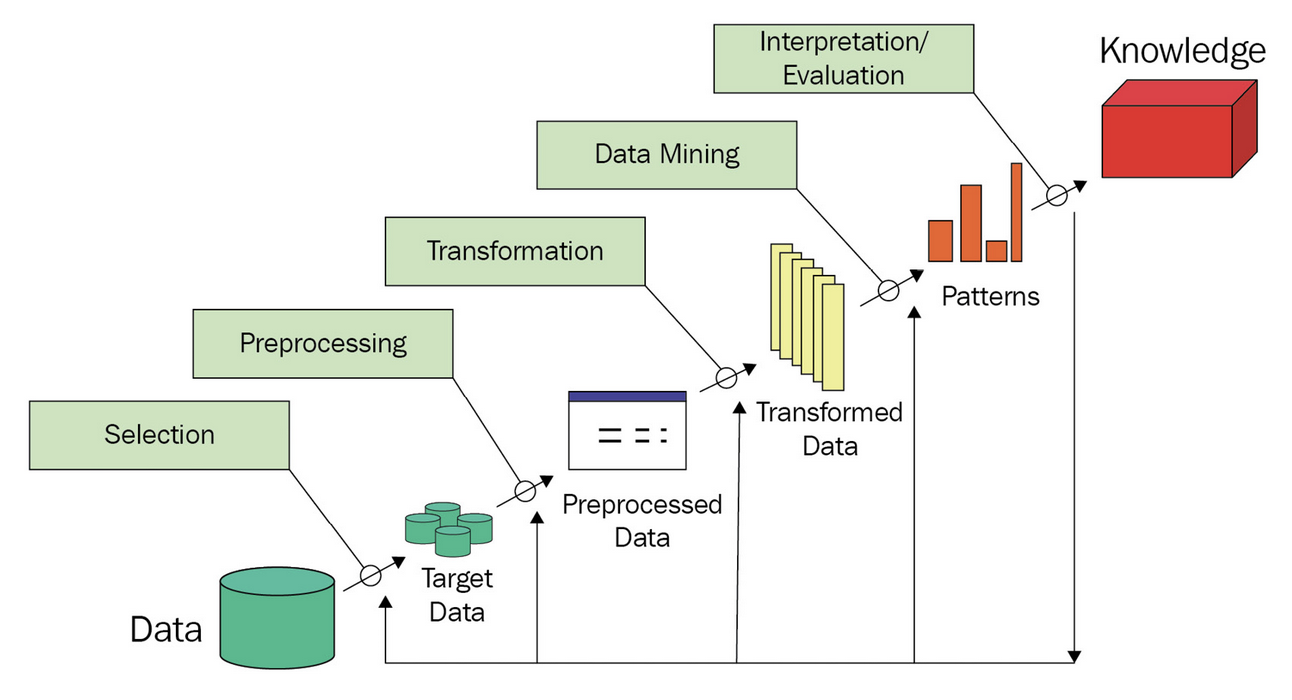
\includegraphics[width=11cm]{Santos_1_6.png}

		\btVFill
		\tiny{Figure from G.R. Santos, Data Wrangling with R.}

	\end{frame}

	\begin{frame}
		\frametitle{Frameworks in Data Science: KDD}

		Knowledge Discovery in Databases

		\vspace{2em}

		\begin{itemize}
			\item Getting the data.
			\item Selecting a subset of samples / variables of interest.
			\item Preprocessing (remove outliers, handle missing or noisy data).
			\item Transformation and formatting.
			\item Data mining (e.g. classification, clustering).
			\item Interpretation and evaluation.
		\end{itemize}

	\end{frame}

	\begin{frame}
		\frametitle{Frameworks in Data Science: SEMMA}

		Sample, Explore, Modify, Model, and Assess

		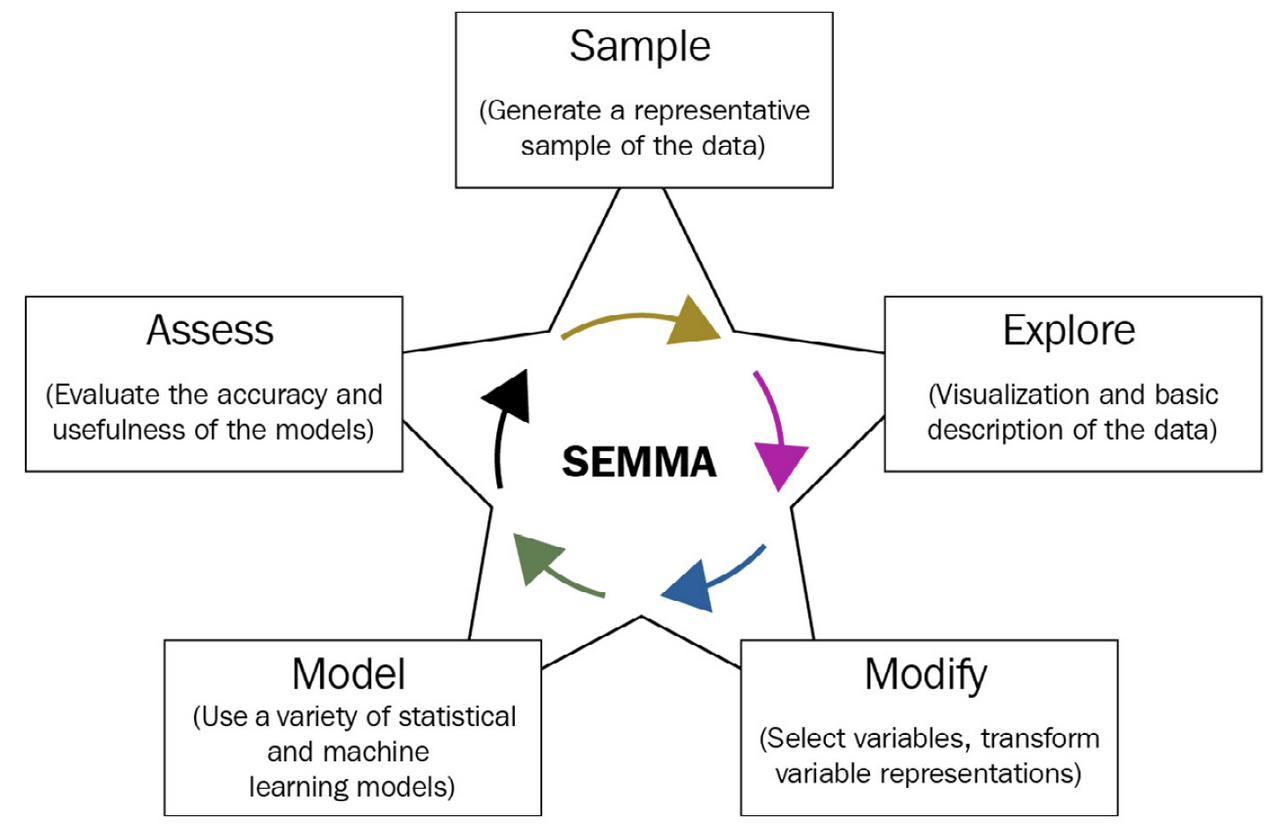
\includegraphics[width=11cm]{Santos_1_7.png}

		\btVFill
		\tiny{Figure from G.R. Santos, Data Wrangling with R.}

	\end{frame}

	\begin{frame}
		\frametitle{Frameworks in Data Science: SEMMA}

		Sample, Explore, Modify, Model, and Assess

		\vspace{2em}

		Cyclic process:
		\begin{itemize}
			\item Sample (representative sample, but easy to work with).
			\item Explore (understand, visualize, describe, patterns and anomalies).
			\item Modify (data wrangling).
			\item Model (algorithms for predictions or insights on the data).
			\item Access (evaluate the results).
		\end{itemize}

	\end{frame}

	\begin{frame}
		\frametitle{Frameworks in Data Science: CRISP-DM}

		Cross-Industry Standard Process for Data Mining

		\begin{center}
		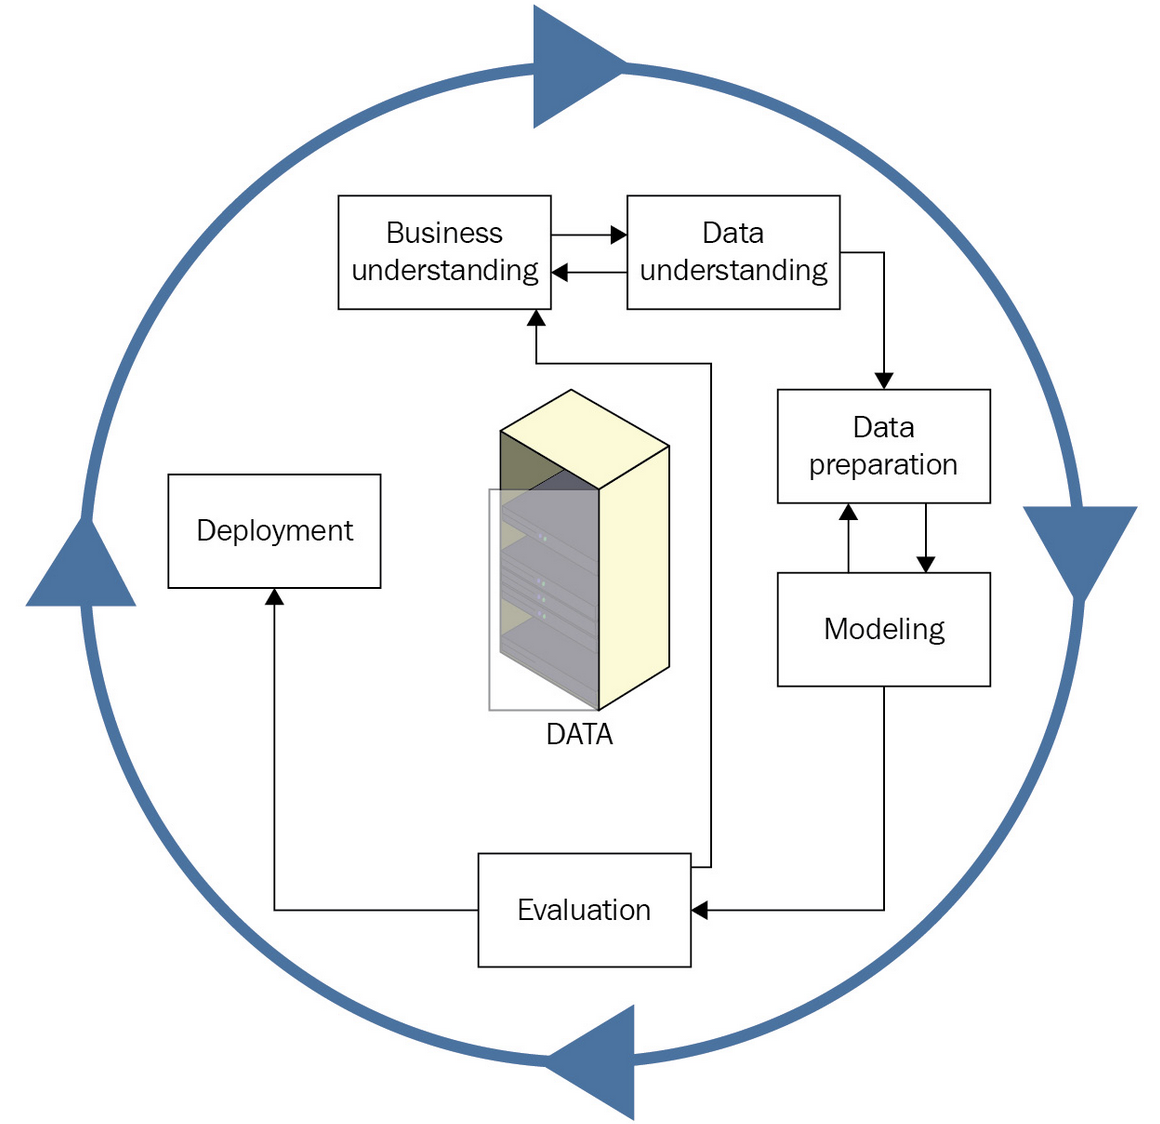
\includegraphics[width=7cm]{Santos_1_8.png}
		\end{center}

		\btVFill
		\tiny{Figure from G.R. Santos, Data Wrangling with R.}

	\end{frame}

	\begin{frame}
		\frametitle{Frameworks in Data Science: CRISP-DM}

		Cross-Industry Standard Process for Data Mining

		\vspace{2em}

		\begin{itemize}
			\item Business understanding: Understand the problem and the business rules and specificities.
			\item Data understanding: Explore the data, find errors and missing data to assess quality.
			\item Data preparation: Data wrangling.
			\item Modeling: Analysis of the processed data.
			\item Evaluation: Assess whether the solution is aligned with the business requirements.
			\item Deployment: The model reaches its purpose.
		\end{itemize}

	\end{frame}
		
	\begin{frame}
		\frametitle{Tibbles versus Data frames}

		\begin{itemize}
		\setlength{\itemsep}{1em}
			\item Tibbles do not change input variable types by default.
			\item Tibbles can have lists as columns.
			\item Tibbles can have non-standard variable names.
			\item Tibbles return another Tibble when slicing (and not a vector).
		\end{itemize}

	\end{frame}

	\begin{frame}[fragile]
		\frametitle{The pipe operator}

		The \verb|magrittr| package provides the $\%<>\%$ operator as a shortcut for modifying an object in place:

		\vspace{1em}

		\begin{exampleblock}{}
		\begin{BVerbatim}
df_iris <- iris %>%
  group_by(Species) %>%
  summarize_if(is.numeric, mean) %>%
  ungroup() %>%
  gather(measure, value, -Species) %>%
  arrange(value)
		\end{BVerbatim}
		\end{exampleblock}{}

		=

		\begin{exampleblock}{}
		\begin{BVerbatim}
df_iris <- group_by(iris, Species)
  df_iris <- summarize_if(df_iris, is.numeric, mean)
  df_iris <- ungroup(df_iris)
  df_iris <- gather(df_iris, measure, value, -Species)
  df_iris <- arrange(df_iris, value)
		\end{BVerbatim}
		\end{exampleblock}{}

	\end{frame}

\end{document}
